\chapter{Circuiti RC e RL (C3)}

Oggetto di studio di questa esperienza è l'andamento della differenza di potenziale ai capi di resistenza e capacità o induttanza.
A tal fine costruiamo un circuito con i seguenti elementi:
[disegno]

\begin{itemize}
  \item Generatore di onde
  \item Un condensatore di capacità 367 $nF$
  \item Un'induttore di induttanza sconosciuta, e resistenza 40 $\Omega$.
  \item Un oscilloscopio con due sonde
  \item Una resistenza di 667 $\pm 10 \Omega$  \footnote{Nel corso dell'esperimento abbiamo verificato, propagando l'errore associato alla resistenza, che esso risultava trascurabile. Pertanto d'ora in poi non se ne terrà più conto}
\end{itemize}

\section{Corrente impulsata}
\subsection{Procedimento}

Per simulare l'apertura e la chiusura del circuito impostiamo nel generatore la modalità onda quadra. Una sonda posta prima del condensatore mostra sullo schermo dell'oscilloscopio il segnale.  
Una seconda sonda, posta ai capi della resistenza, visualizza la forma dell'onda caratteristica della carica o della scarica di un condensatore/induttore.

\subsubsection{Circuito RC}

Raccogliamo i dati (differenza di potenziale e tempo) dall'onda visualizzata sul display dell'oscilloscopio, tramite i cursori. 

Con un'onda quadra a 50 Hz, abbiamo raccolto i seguenti dati:
\begin{center}
\begin{tabular}{*{2}{c}}
Tempo ($\mu s$) & Ddp ($V$) \\
\midrule
0 & 18.20 \\
100 & 12.80 \\
200 & 9.00 \\
300 & 5.80 \\
400 & 4.40 \\
500 & 3.20 \\
600 & 2.20 \\
700 & 1.80 \\
800 & 1.20 \\
900 & 1.00 \\
\end{tabular}
\end{center}

Interpoliamo i dati raccolti con la curva caratteristica della carica di un condensatore: 
$$V_R = \varepsilon e^{-t/\tau}$$

Il valore stimato dall'interpolazione è $\tau=281.7 \pm 5 \mu s$.
Valore atteso: $\tau=RC=248.5 \mu s$

Otteniamo un valore: $\chi^2 = 70 $. Dati 7 gradi di libertà, $\tilde{\chi}^2 = 10$.


\begin{center}
 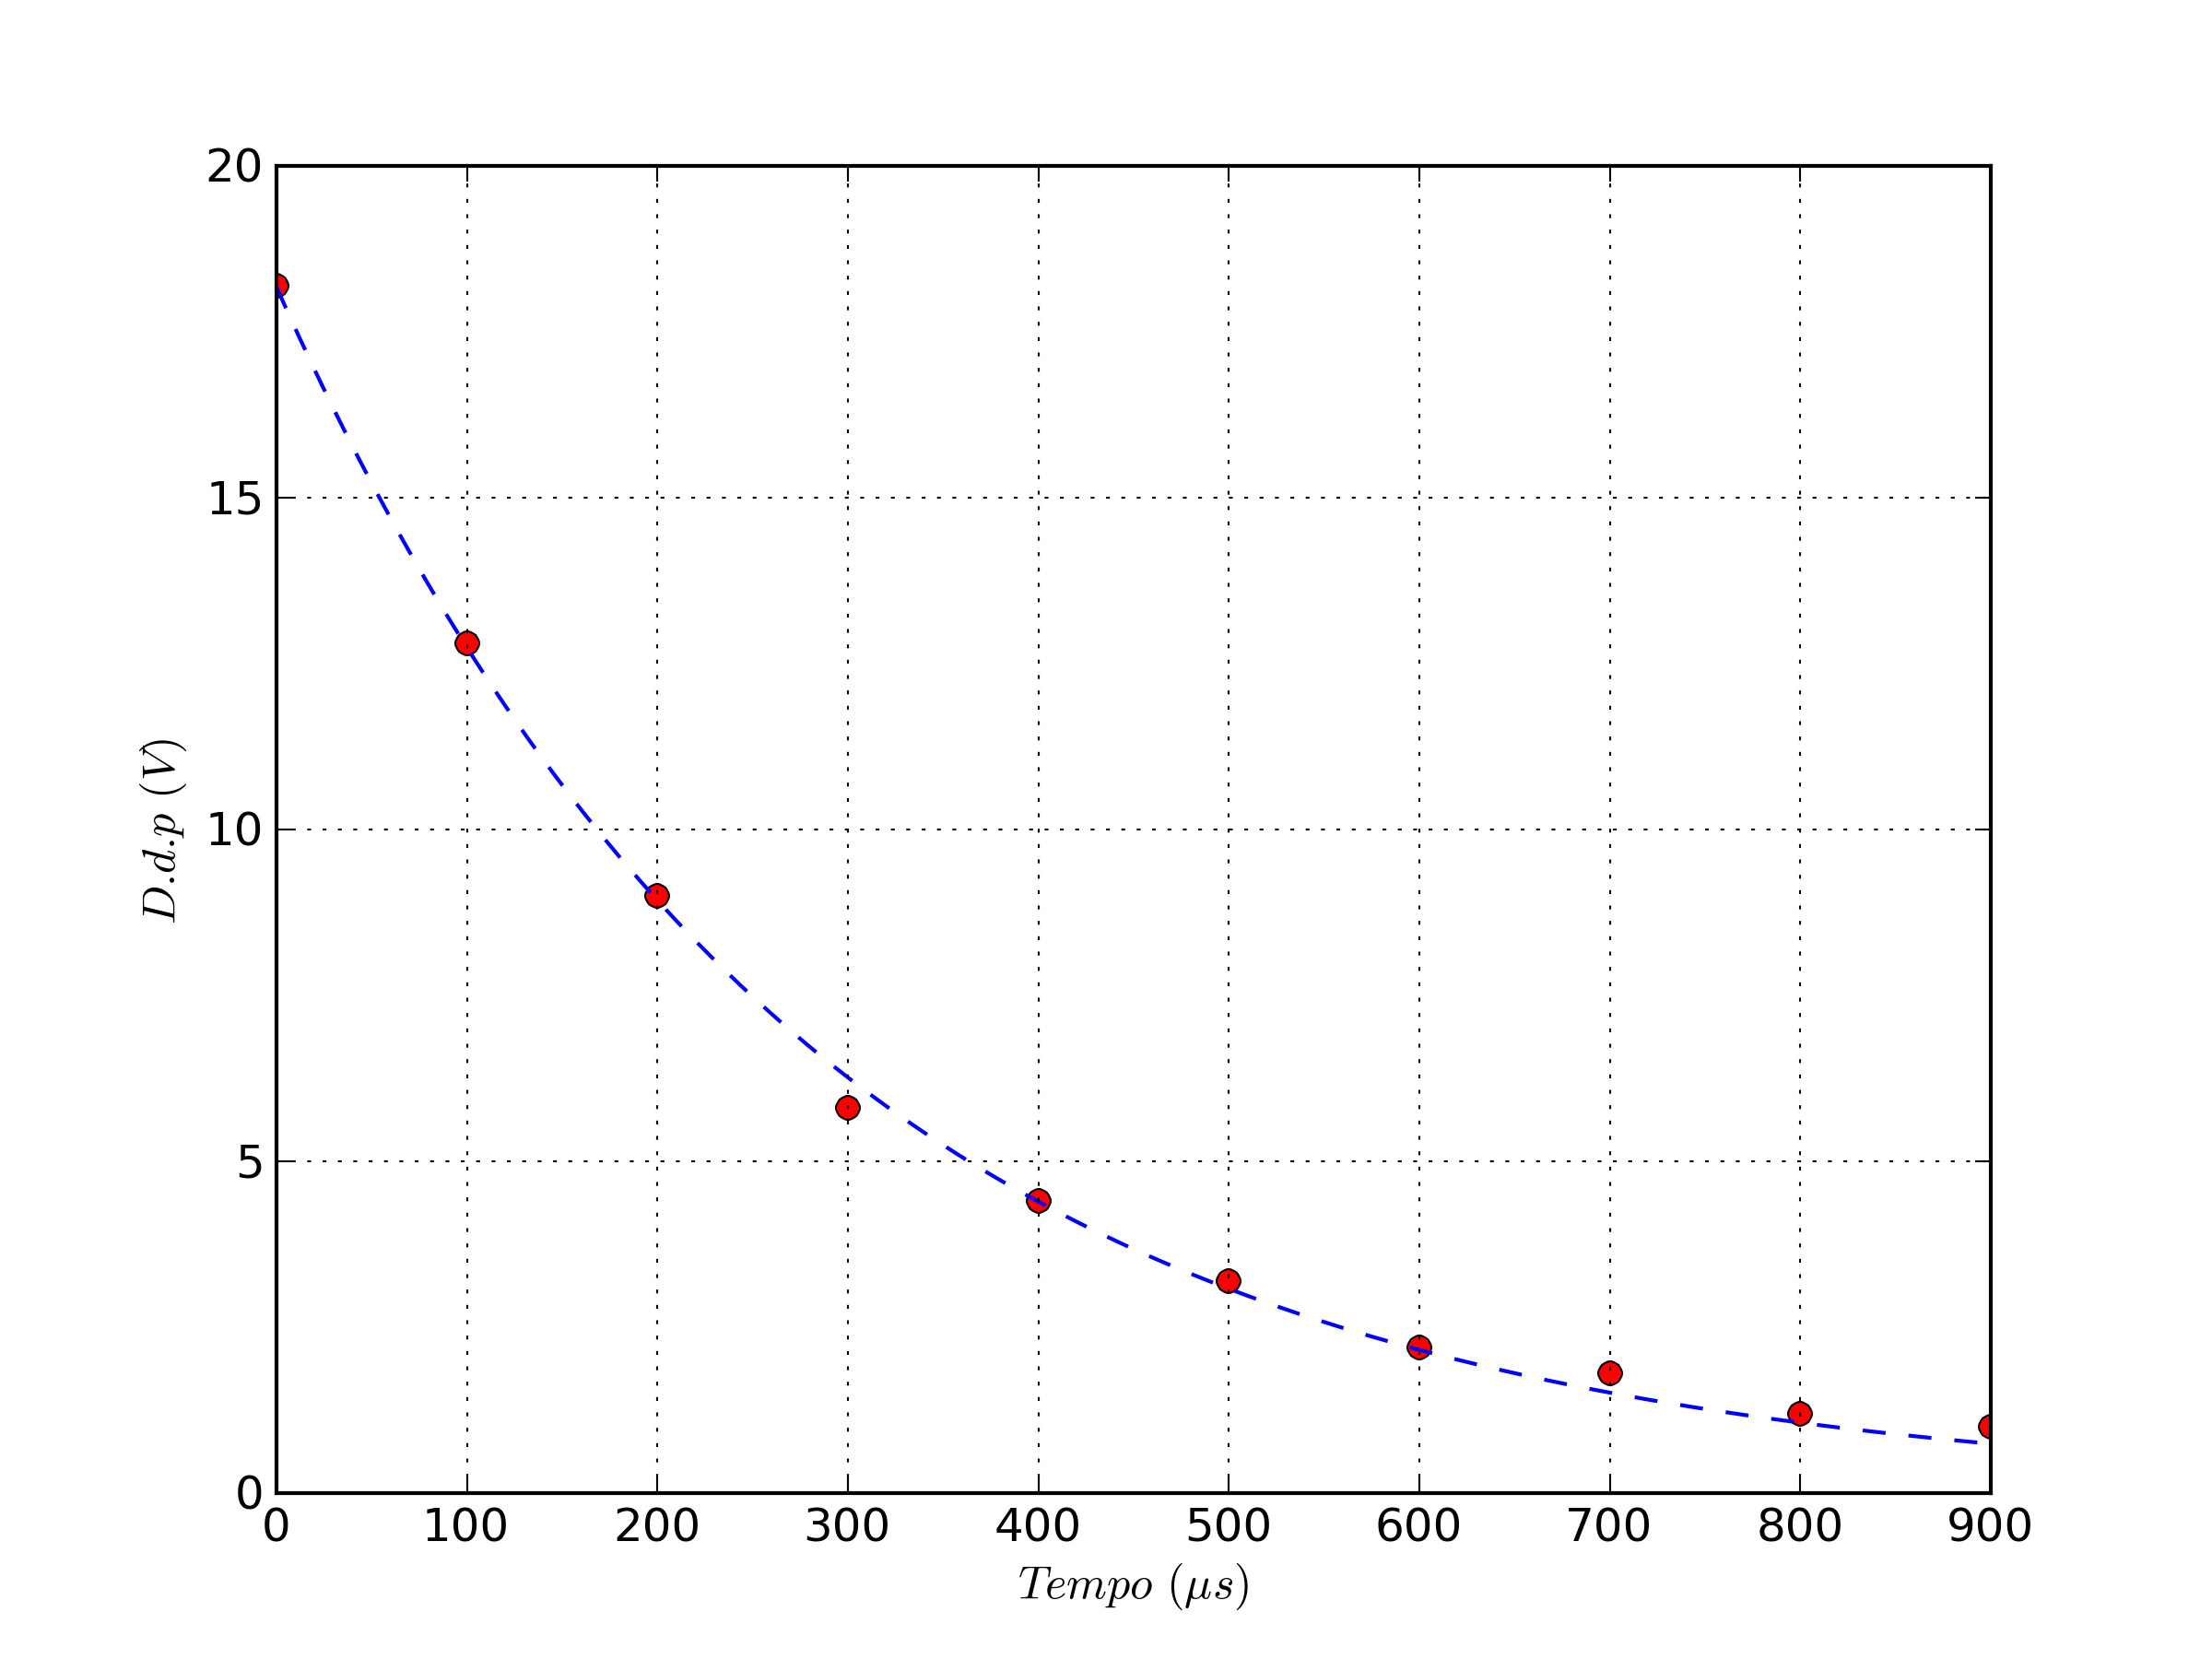
\includegraphics[scale=0.70]{grafici/C3/fitcond.png}
\end{center}

Per verificare l'accordo tra la legge e la distribuzione dei valori osservati operiamo il test del $\chi^2$, nella forma:

$$ \chi^2 = \frac{\sum{(y_i - f(x_i,\tau )}}{\sigma_y^2} $$

\subsubsection{Circuito RL}
Con un'onda quadra a 250 Hz, abbiamo raccolto i seguenti dati:

\begin{center}
\begin{tabular}{*{2}{c}}
Tempo ($\mu s$) & Ddp ($V$) \\
\midrule
5 & 5.00 \\
10 & 8.00 \\
15 & 10.60 \\
20 & 12.40 \\
25 & 13.60 \\
30 & 14.60 \\
35 & 15.40 \\
40 & 16.20 \\
45 & 16.40 \\
\end{tabular}
\end{center}
Interpoliamo i dati raccolti con la curva caratteristica della carica del circuito:

$$V_R = \varepsilon \left( 1-e^{-t/\tau} \right)$$

Il valore stimato dall'interpolazione è $\tau=16.05 \mu s$ \\
Non conoscendo a priori il valore di L non possiamo valutare l'accordo con il valore teorico: $\tau=\frac{L}{R}$.

\begin{center}
 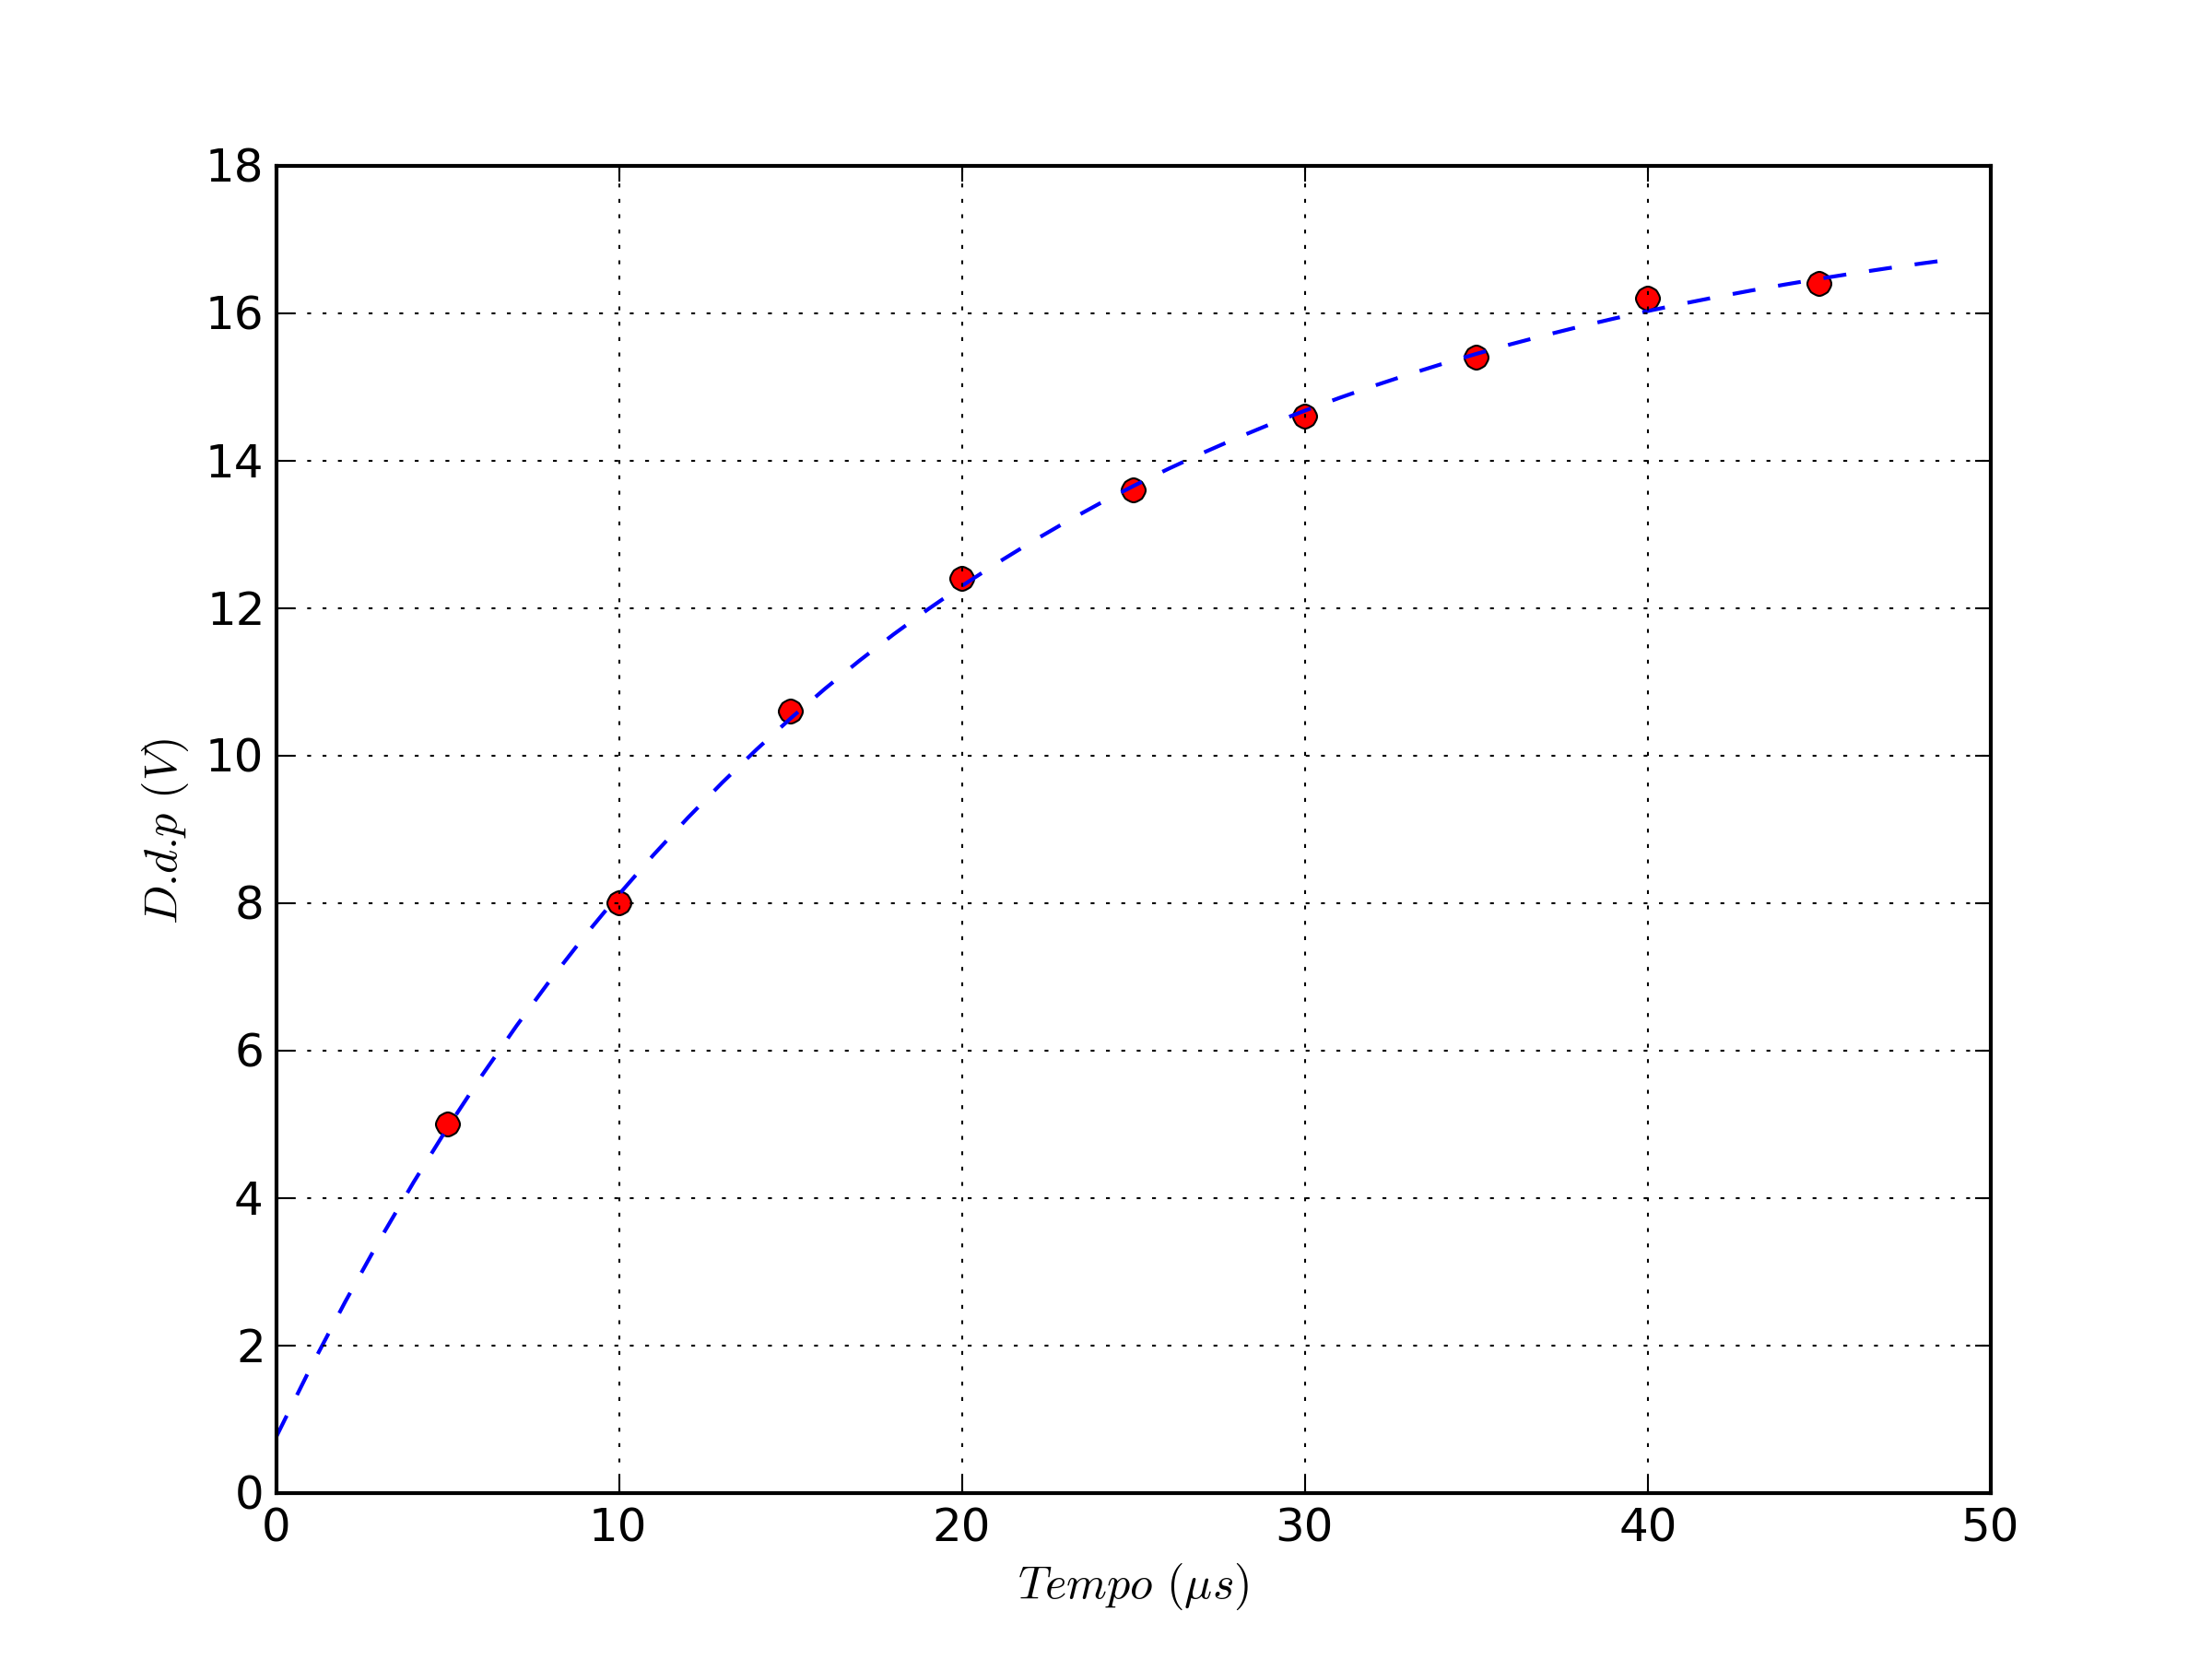
\includegraphics[scale=0.70]{grafici/C3/fitindu.png}
\end{center}

Otteniamo un valore: $\chi^2 = 0,.38 $. Dati 7 gradi di libertà, $\tilde{\chi}^2 = 0.05$.


\section{Corrente alternata}
\subsection{Procedimento}
Nella seconda parte dell'esperienza intendiamo misurare la risposta in frequenza (o funzione di trasferimento), definita come:

$H\left(\omega \right) = $  


Pertanto misuriamo la ddp ai capi di $R$ e $C$ o $L$ in modo analogo alle prima parte dell'esperienza, e la distanza tra due picchi delle onde visualizzate a schermo per determinare l'angolo $\phi$ di sfasamento ($\delta \phi = 2 \pi \delta t \ni$).

Per ricavare il rapporto $\frac{V_{R}}{V_{o}}$, dobbiamo ricavare $V_R$. Trovandoci in regime di corrente alternata, la leggge di Ohm è nella forma: $ V_o = Zi_o$ con $Z = R + jX$, impedenza del circuito.
Trattandosi di circuiti RC e RL in cui le impedenze sono collegate in serie, si ha $Z_{tot} = \sum Z_i$

\begin{itemize}
\item circuito RC $\rightarrow$ $Z=R-\frac{j}{\omega C}$
\item circuito RL $\rightarrow$ $Z=R+j\omega L$
\end{itemize}  

Allora: 

$$V_{Ro} = Ri_o = \frac{V_o}{Z} = \frac{RV_o}{\sqrt{R^2+X^2}} $$ 
75fa

\begin{itemize}
\item circuito RC $\rightarrow$ $X=\frac{1}{\omega C}$
\item circuito RL $\rightarrow$ $X=\omega L$
\end{itemize}

Mentre la fase risulta: 
$$\phi = \arctan \frac{X}{R} $$


\subsection{Circuito RC}


\begin{center}

\begin{tabular}{*{3}{c}}
Frequenza ($Hz$) & Delta V ($V_{out}/V_{in}$) & $\phi$ \\
\midrule
50 & 0.08 & 1.54\\
100 & 0.15 & 1.41\\
200 & 0.30 & 1.41\\
300 & 0.42 & 1.24\\
400 & 0.52 & 1.08 \\
1000 & 0.83 & 0.70\\
1500 & 0.90 & 0.49\\
2000 & 0.93 & 0.38\\
4000 & 0.97 & 0.20 \\
\end{tabular}
\end{center}

Lasciamo C come parametro libero, e interpoliamo i valori raccolti di $V_{out}$ e $V_{in}$ in funzione della frequenza:

$$\frac{V_{Ro}}{V_o} = \frac{R}{\sqrt{R^2+(\omega C)^{-2}}}$$

Dal fit otteniamo: $C=360 \cdot 10^{-9} \pm  F $ in ottimo accordo con il valore noto.

\begin{center}
 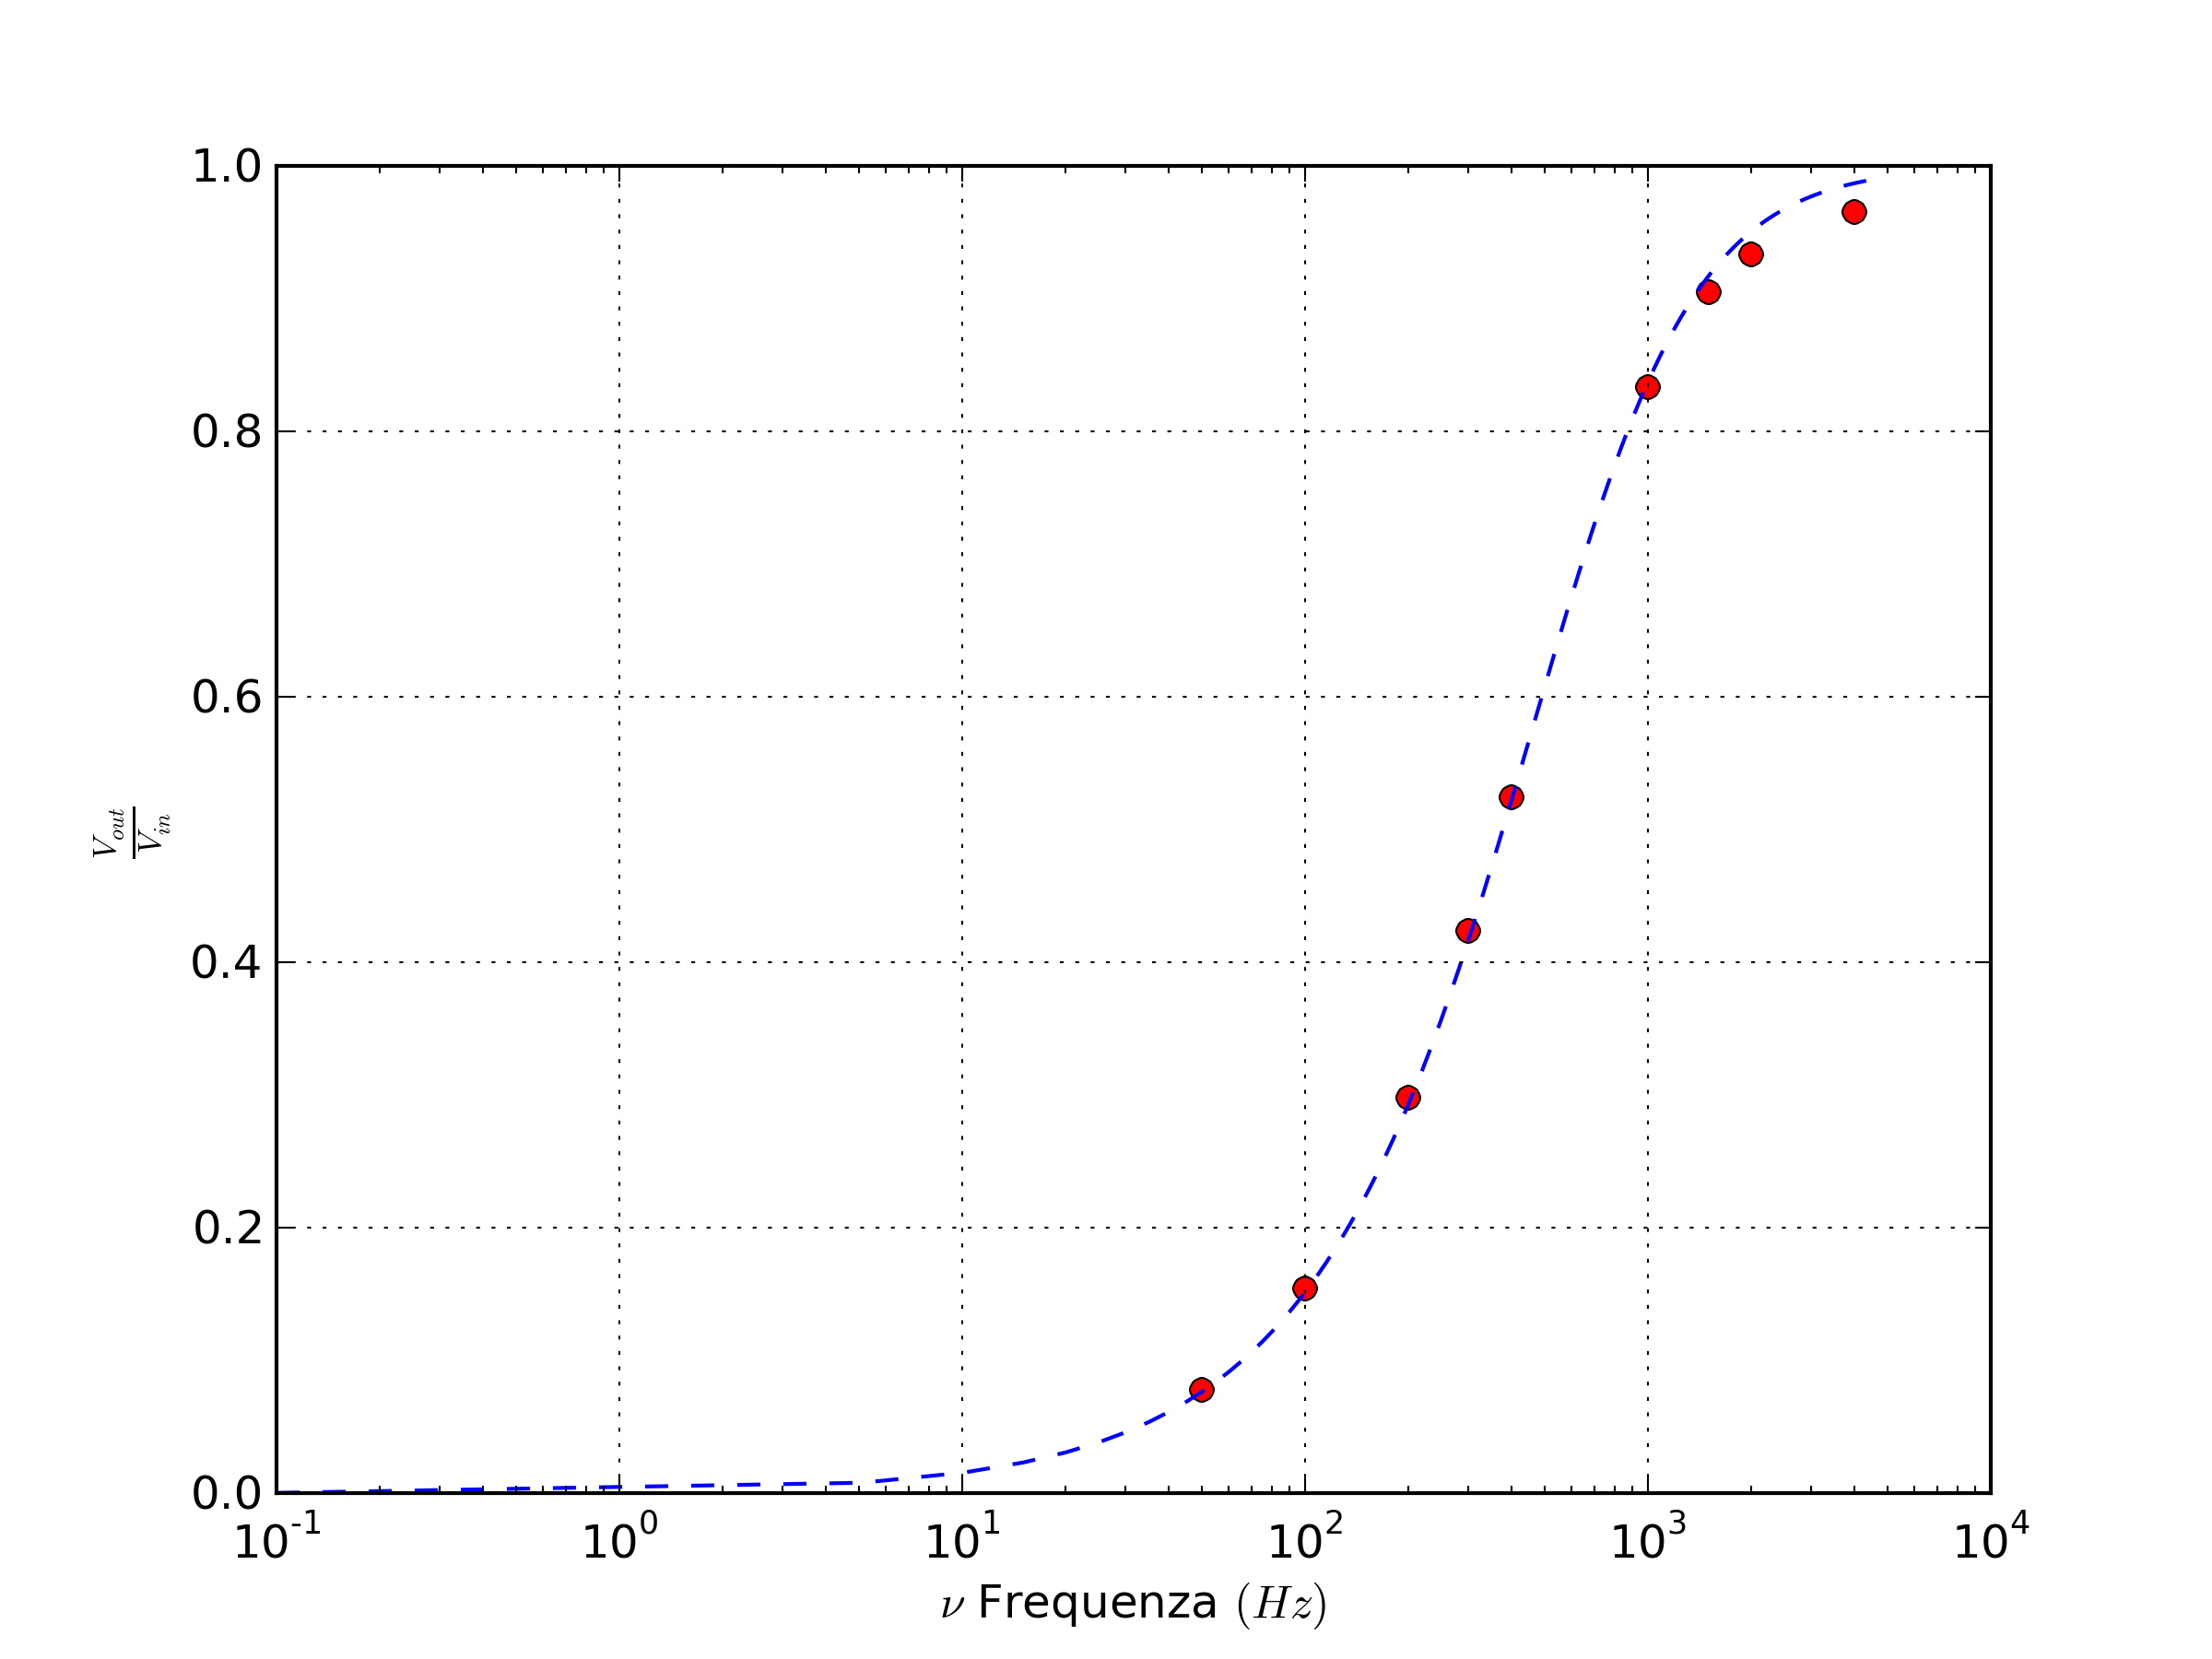
\includegraphics[scale=0.70]{grafici/C3/ddpcond.png}
\end{center}

\begin{center}
 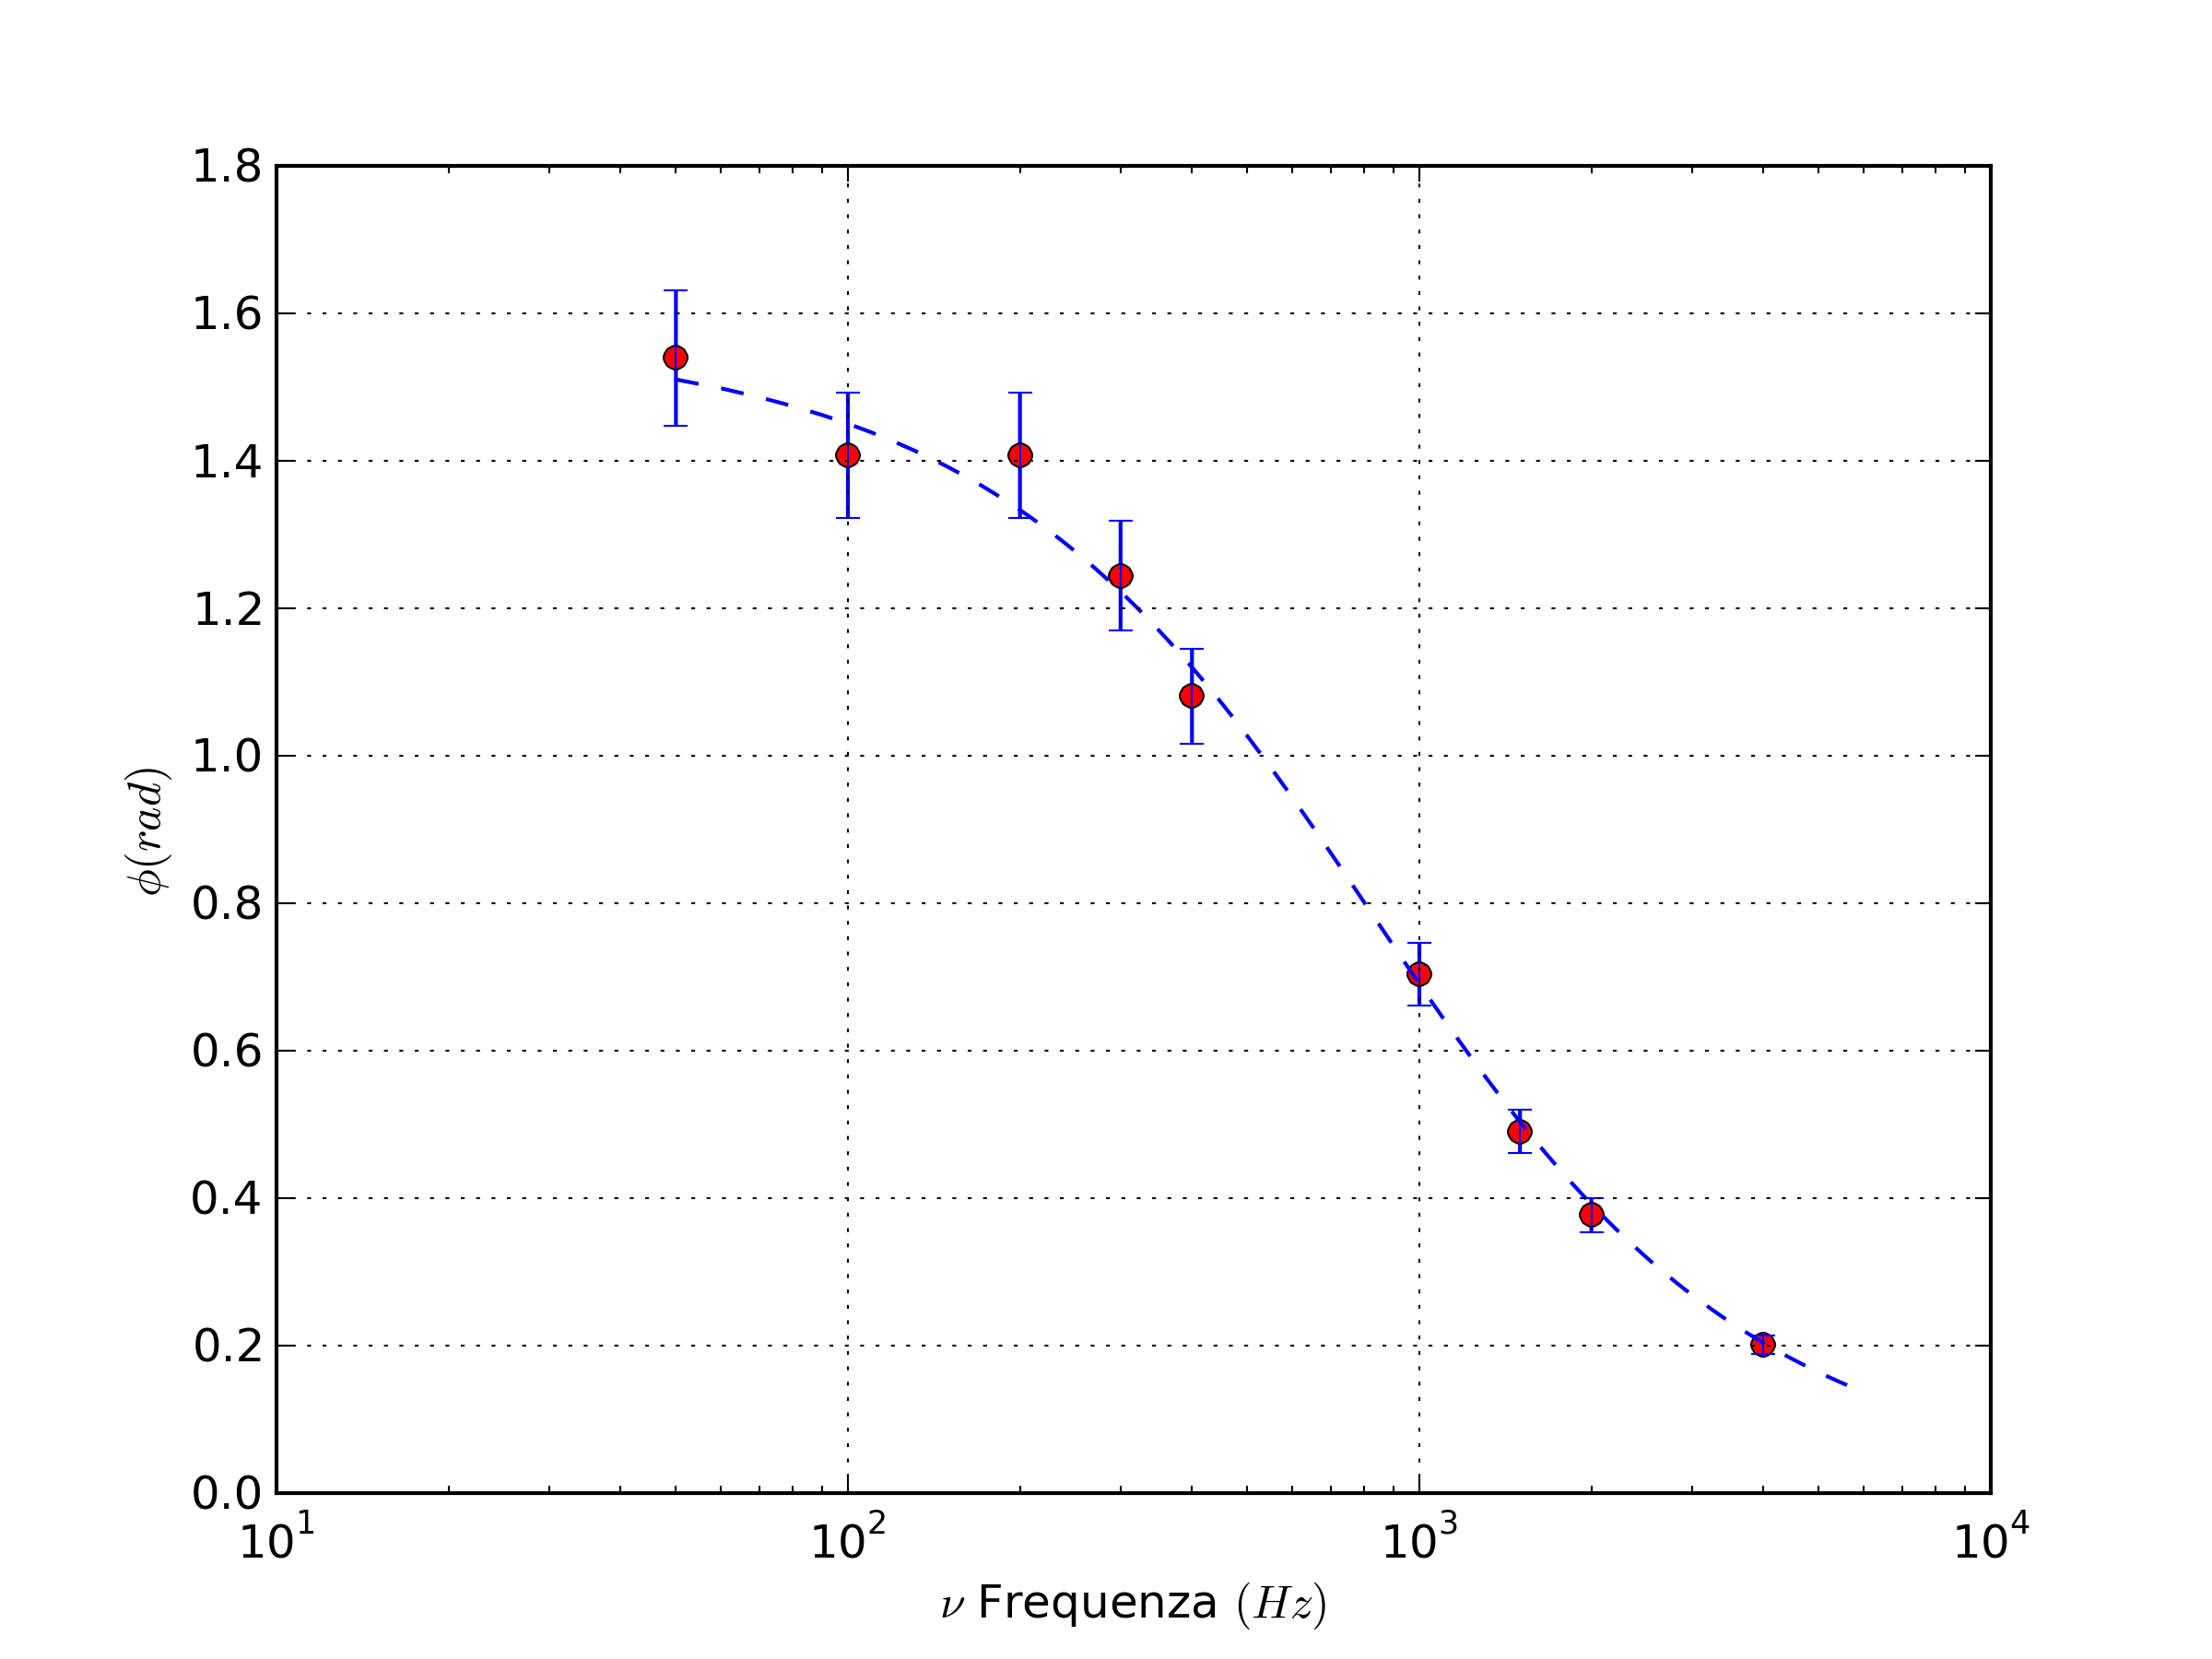
\includegraphics[scale=0.70]{grafici/C3/fasecap.png}
\end{center}



Interpolo i dati della $\delta \phi$ utilizzando la funzione:

$$ \phi = \arctan \frac{1}{2\pi\nu C R} $$

con C parametro libero. Tramite il test del $\chi^2$ verifico l'accordo con i nostri dati, ottenendo un $\tilde{\chi}^2 = 1.05$

\subsection{Circuito RL}
\begin{center}

\begin{tabular}{*{3}{c}}
Frequenza ($Hz$) & Delta V ($V_{out}/V_{in}$) & $\phi (rad)$ \\
\midrule
1000& 0.47 & 0.19 \\
2000 & 0.62 & 0.35\\
3000 & 0.79 & 0.45\\
4000 & 1.05 & 0.58\\
6000 & 1.48 & 0.79\\
8000 & 2.01 & 1.01\\
10000 & 2.56 & 0.94\\
15000 & 3.64 & 1.13\\
20000 & 4.28 & 1.26\\
30000 & 5.08 & 1.36\\
50000 & 5.89 & 1.57\\
\end{tabular}
\end{center}


\begin{center}
 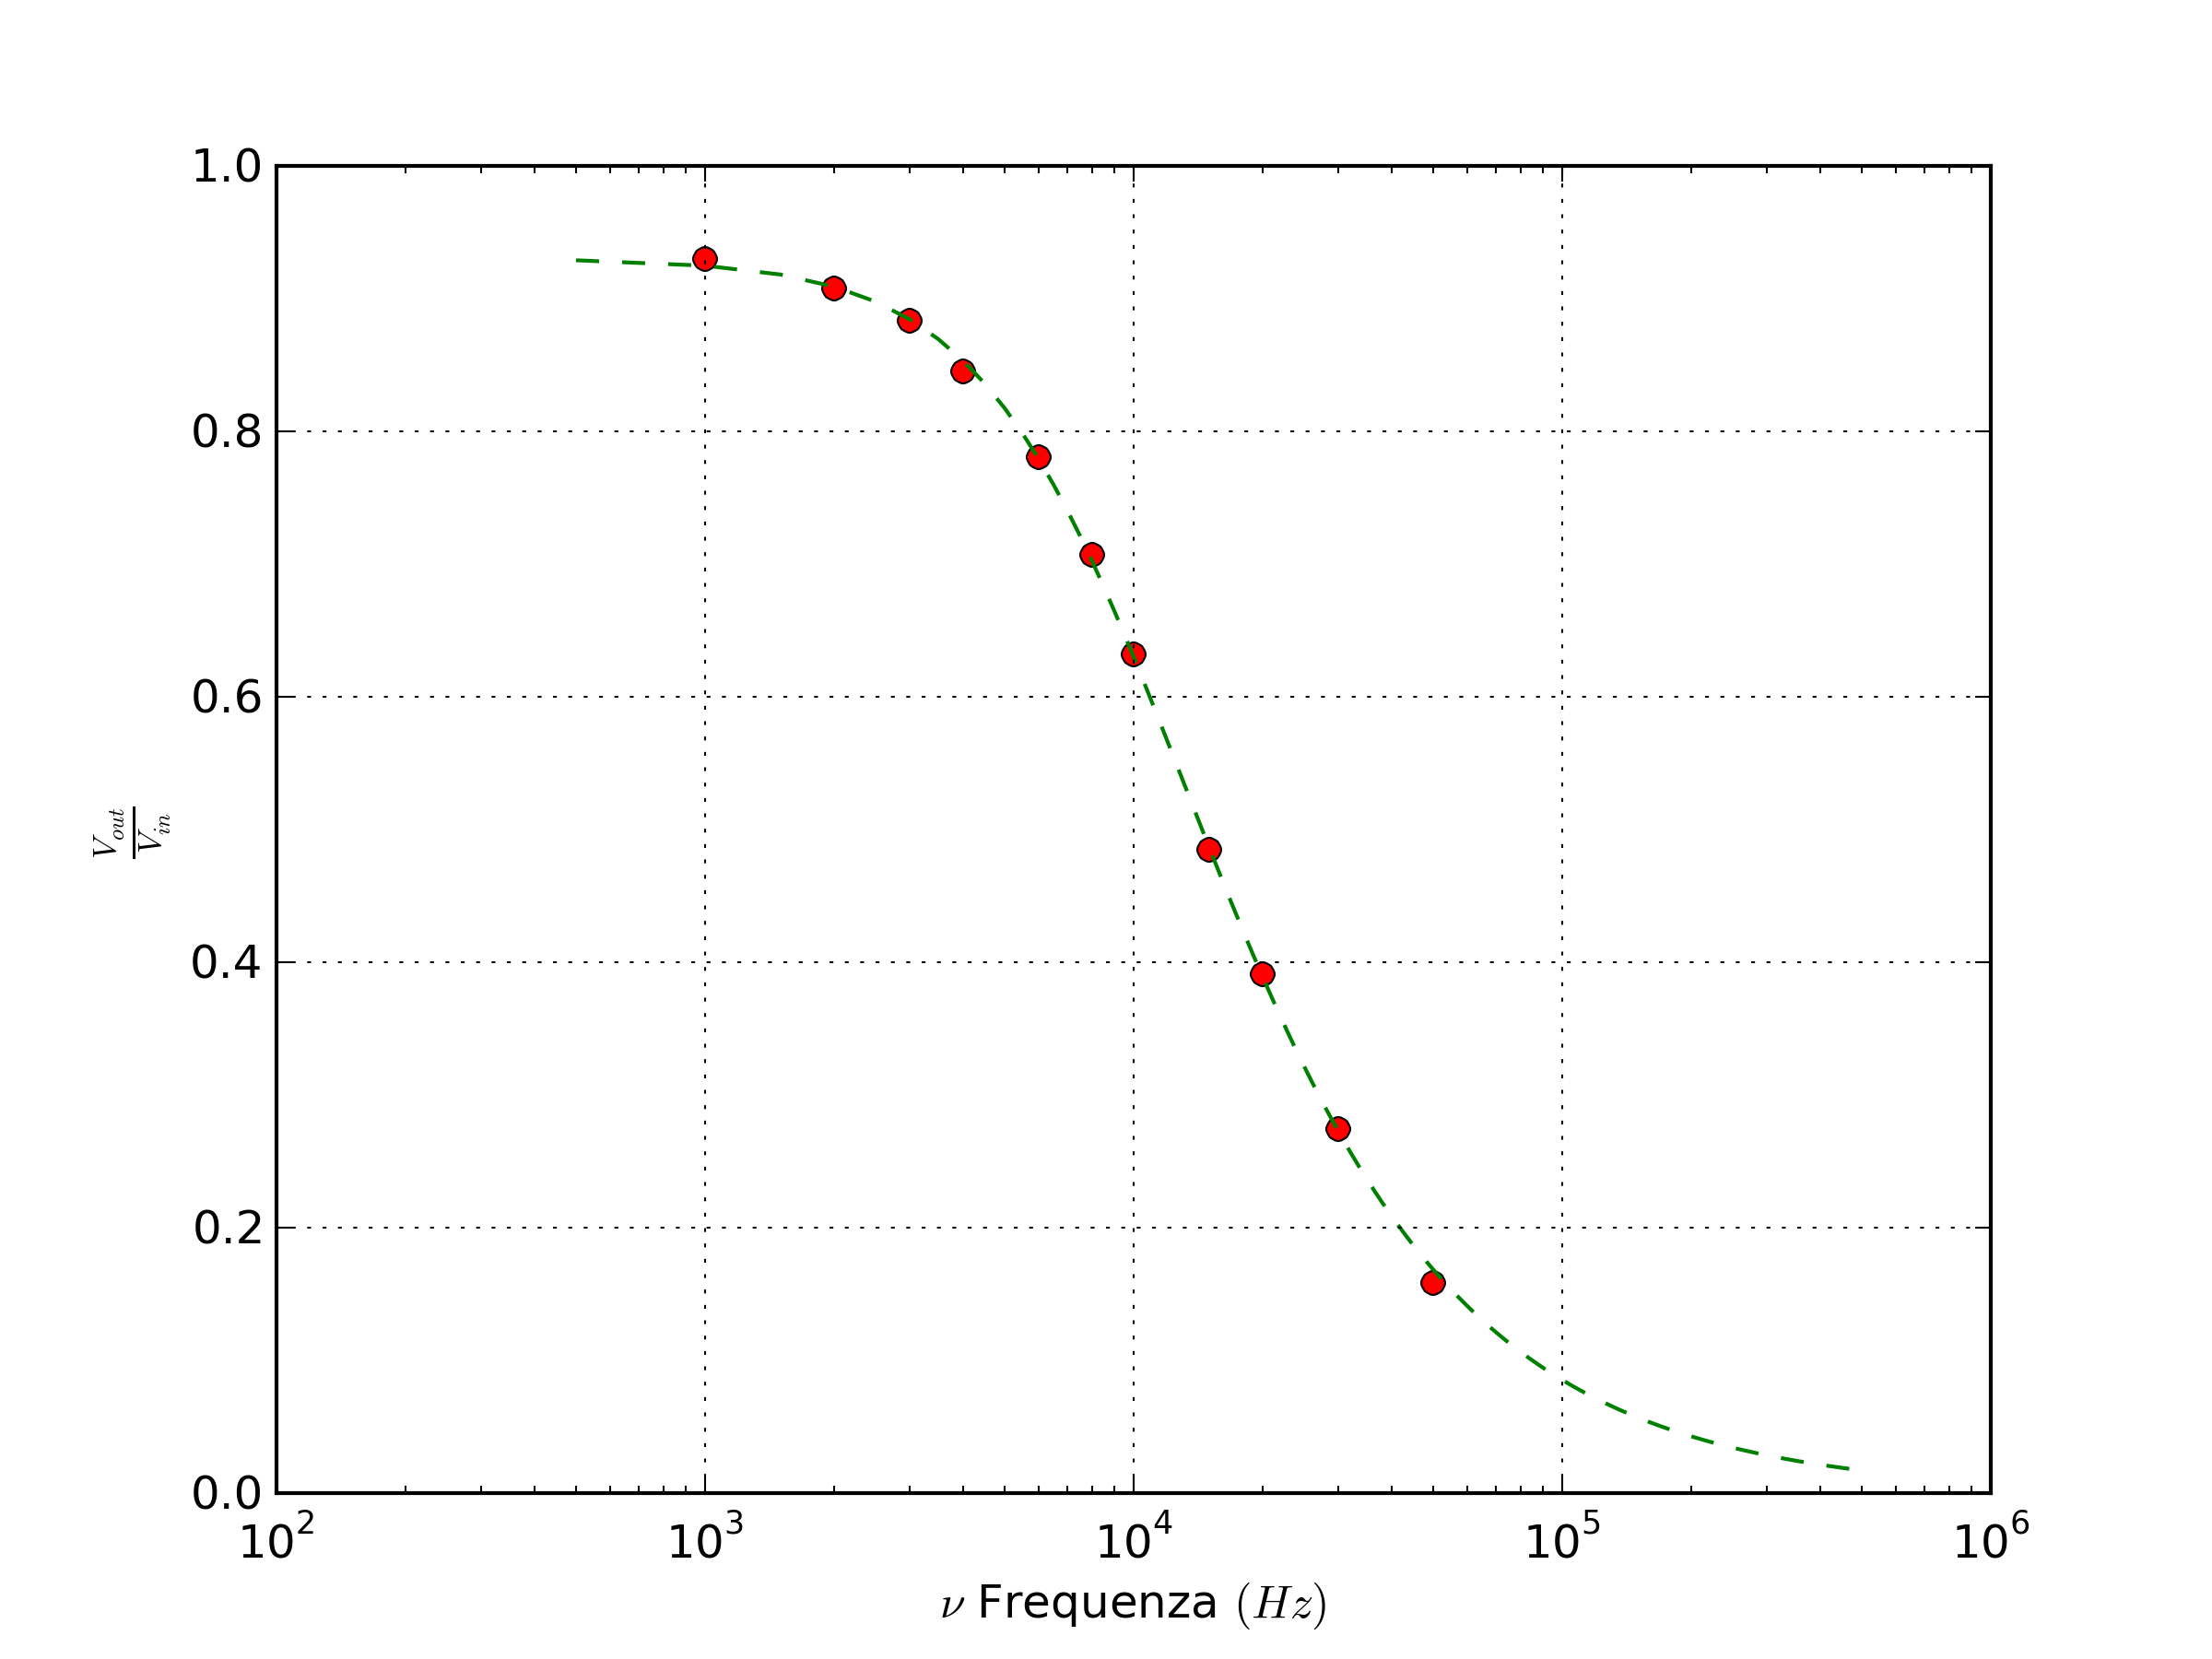
\includegraphics[scale=0.70]{grafici/C3/ddpindu.png}
\end{center}

Anche questa volta interpoliamo i dati raccolti con la funzione:

$$\frac{V_{Ro}}{V_o} = \frac{R}{\sqrt{R^2+(\omega L)^2}}$$

La stima di L risulta in ottimo accordo con quella realizzata nella prima parte dell'esperienza.
$L=0.0012 \pm H $

Il test del $\chi^2$ conferma la validità delle ipotesi fatte.

(chi quadro della delta phi 0.96)


Interpolo i dati utilizzando la funzione:

$$ \phi = \arctan \frac{2\pi\nu L}{R} $$

dove L, è il parametro libero da stimare.


\begin{center}
 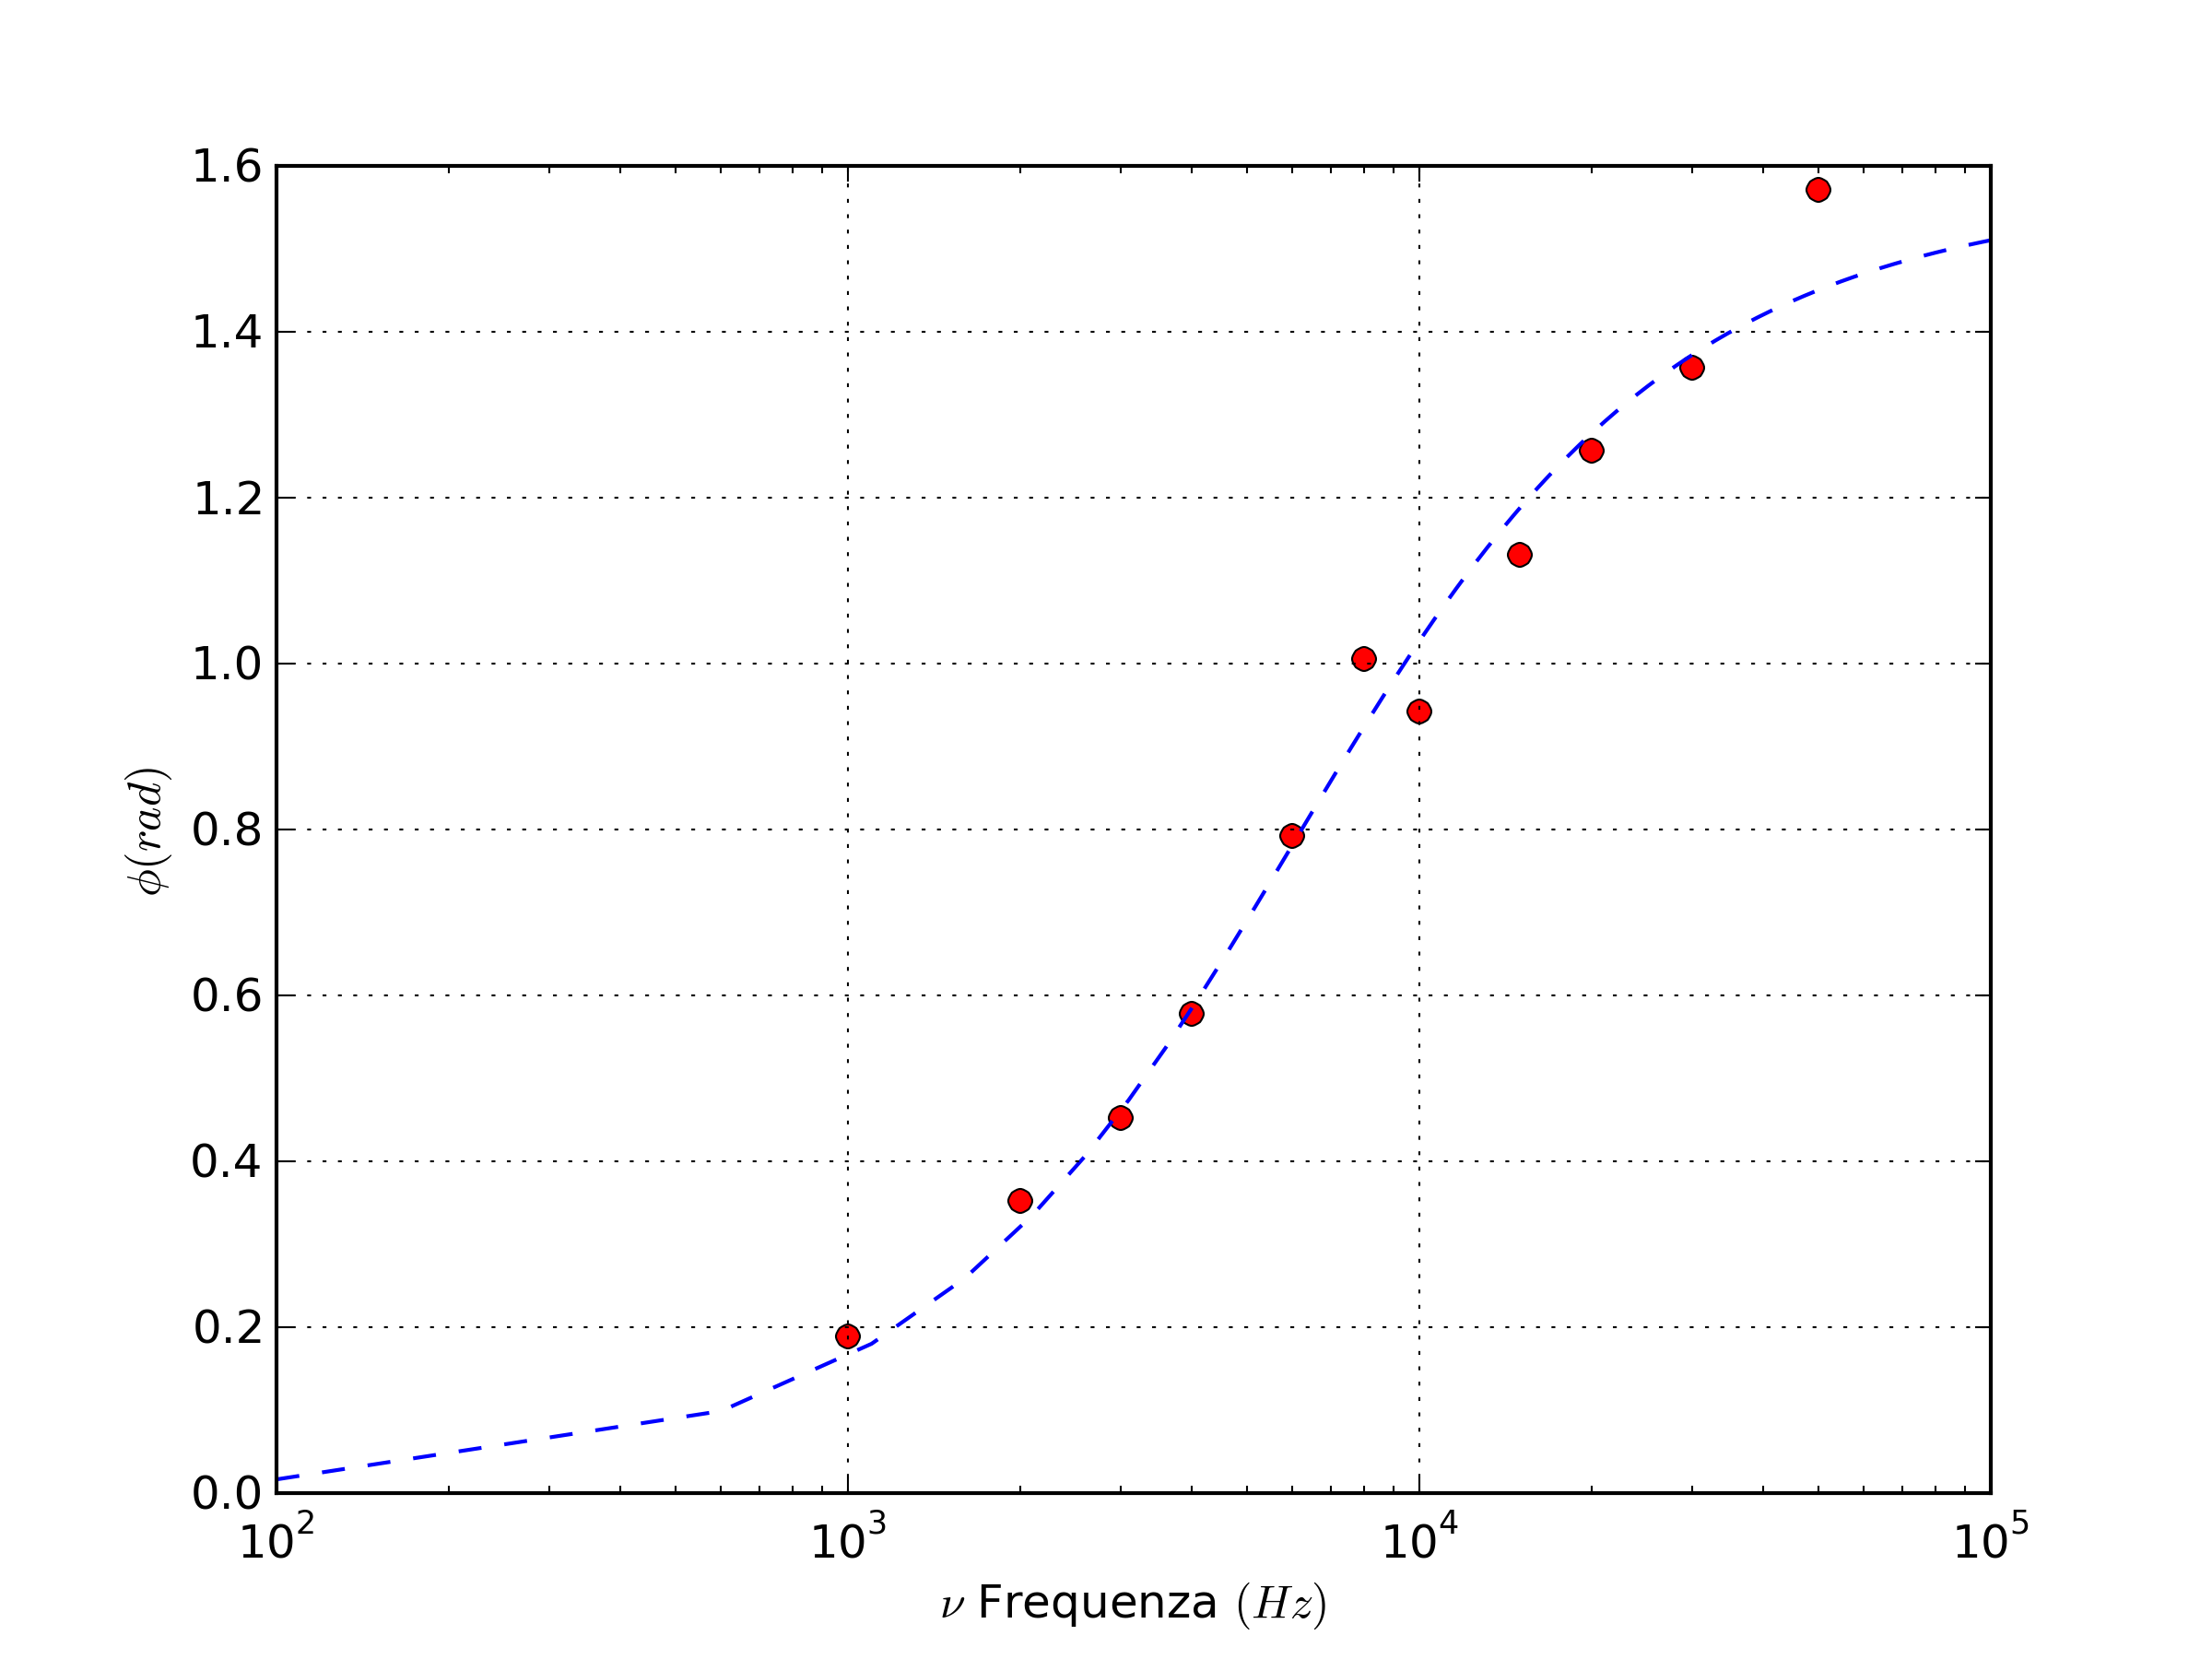
\includegraphics[scale=0.70]{grafici/C3/faseindu.png}
\end{center}

Da questo fit, otteniamo una $L=0.0017 H$, e un $\chi^2 = 8.48 $, considerando una $\sigma_y_i = 2 \pi \nu_i \sigma_{t}$, dove  per $\sigma_t = \pm 2 \mu s$. L'incertezza sulla frequenza è trascurabile, e per questo motivo abbiamo propagato l'incertezza solo su $\sigma_t$. Poichè $\sigma_i$ è proporzionale alla frequenza, l'incertezza della misura di $\phi$ sulle frequenze più elevate diviene dunque rilevante rendendo possibile accettare un $\chi^2$ così piccolo, pur per un fit che, graficamente, non sembra in buon accordo. Il grafico è inoltre logaritmico, e accentua questo effetto. 

Poichè abbiamo 9 gradi di libertà, otteniamo un $\tilde{\chi}^2 = 0.94$.
 

\section{Conclusioni}


\begin{center}
\begin{tabular}{*{2}{c}}
Parametro & $\chi^2$ \\
\midrule
Condensatore $\tau =$ & 0.2 \\
Induttore $\tau =$ & 0.2 \\

\end{tabular}
\end{center}

